\chapter{Lavorazioni per asportazione di truciolo}\label{chp:AsportaTruciolo}
Il principio di funzionamento delle lavorazioni per asportazione di truciolo è
differente da quanto visto fin ora.
Nelle lavorazioni per deformazione plastica si avevano delle deformazioni lente.
\emph{"Per cui il materiale aveva il tempo di adattarsi"}.
Per l'asportazione di truciolo così non può essere. Infatti si suppone che il
materiale venga rotto, tra l'altro il più rigidamente possibile.
Dunque le deformazioni richieste devono essere a più alta velocità.
Ciò però crea delle problematiche non indifferenti:
\begin{itemize}
\item deformazioni veloci non sono rappresentabili tramite prove classiche.
\item Si rende necessario idealizzare il processo e man mano aggiungere ipotesi più realistiche.
\end{itemize}

\section{Introduzione}
Nelle lavorazioni viste fin ora si portava il materiale a deformazione, anche per la tranciatura
nel momento in cui il materiale subiva una deformazione critica fino all'innesco di cricche da cui poi
avveniva la separazione del materiale.
Per l'asportazione del truciolo non può essere così: la deformazione avviene in tempi molto più rapidi,
per cui il materiale ha comportamenti differenti da quelli visti in precedenza.
Inoltre, considerando il materiale di scarto, per le lavorazioni a deformazione si può recuperare ed 
eventualmente riciclare.
Per le lavorazioni ad asportazione la cosa è molto più complicata e difficile.
Il valore del truciolo è pressoché nullo e il suo recupero può essere complicato 
per via delle molteplici varietà di materiale che possono subire tali lavorazioni.
Alla tabella \ref{examp:VantSvant} sono riportati alcuni vantaggi e svantaggi di tali lavorazioni.

\begin{example}{Vantaggi e Svantaggi}
\centering
\begin{tabularx}{\textwidth}{XX}
\toprule
\textbf{Vantaggi} & \textbf{Svantaggi}\\
\midrule
Si possono ottenere tolleranze migliori & Tempo ciclo molto più lento\\
\midrule
Buona finitura superficiale & Scarti di materiale non recuperabili\\
\midrule
\multicolumn{2}{c}{Adatti alla lavorazione di pezzi unici}\\
\midrule
Costo macchina relativamente basso & Spesso è richiesta alta lavorazione manuale\\
\bottomrule
\end{tabularx}
\label{examp:VantSvant}
\end{example}

In industria si sta cercando di eliminare queste lavorazioni per via del tempo ciclo molto elevato.
Sebbene, in abito artigianale stiano avendo un forte sviluppo, sia in termini di automazione,
dunque di tecnologia a bordo macchina; sia di lavorazioni permesse dalle macchine.
Altro grande punto a favore di tali lavorazioni è sicuramente l'adattabilità per 
qualsiasi materiale.

In industria, vengono relegate ad operazioni di finitura del prodotto, dove con una
singola passata si cerca di completare il prodotto e metterlo sul mercato.
Per l'artigianato invece si ha un utilizzo più intensivo, dove con una passata si cerca 
di ottimizzare la quantità di materiale asportato.

Come punto di partenza è utile considerare applicazioni in cui il processo sia completamente
idealizzato.

\section{Taglio ortogonale ideale}
Alla figura \ref{fig:TaglioOrto} sono rappresentati degli esempi di taglio ortogonale.

\begin{figure}
\centering
\subfloat[][\emph{Visualizzazione del taglio ortogonale}\label{fig:TaglioOrto}]
{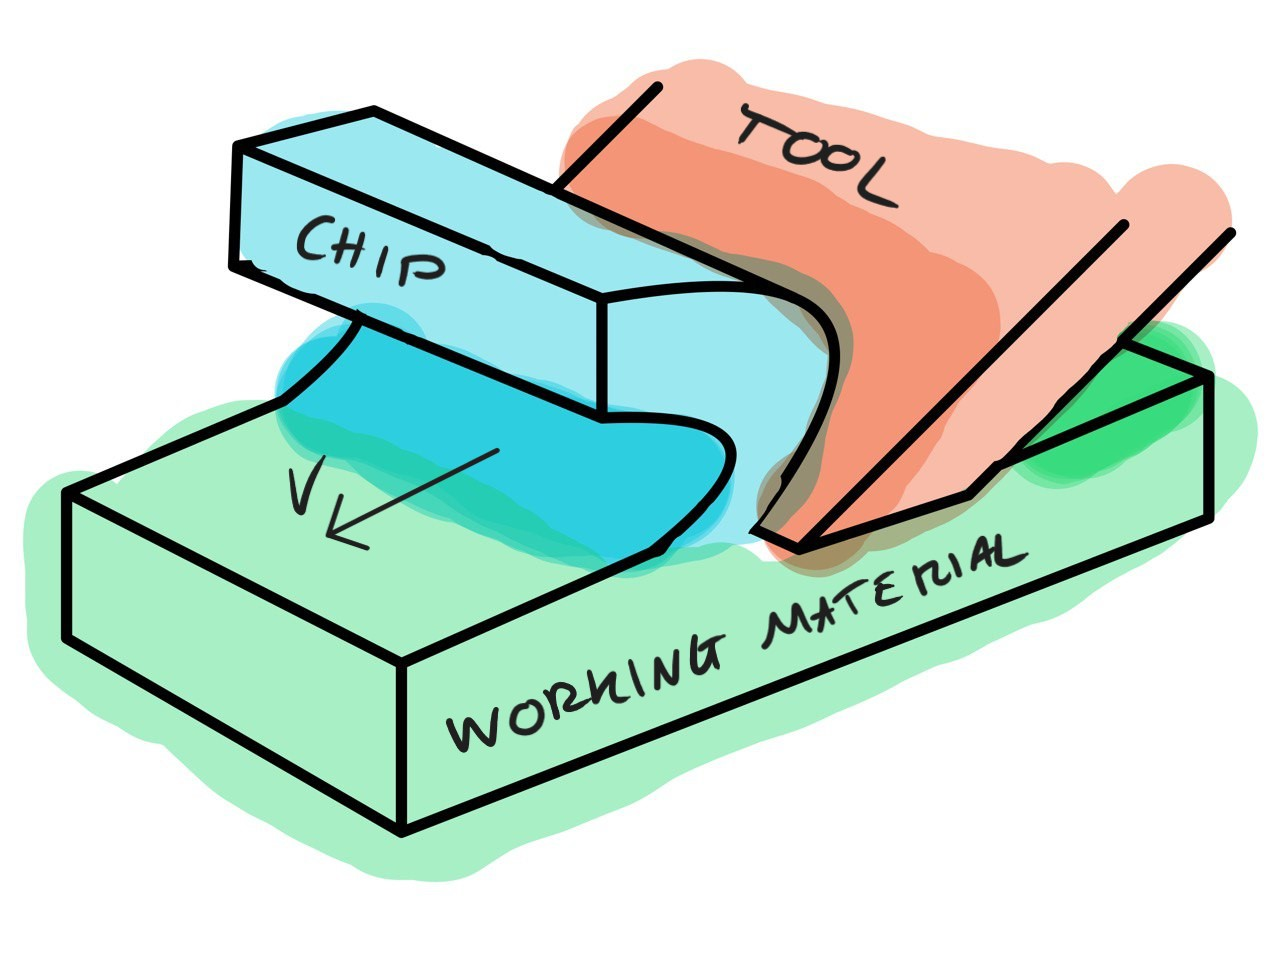
\includegraphics[width = 0.8\textwidth]{TaglioOrto}}\\
\subfloat[][\emph{Parametri del taglio ortogonale}\label{fig:TaglioOrtoParam}]
{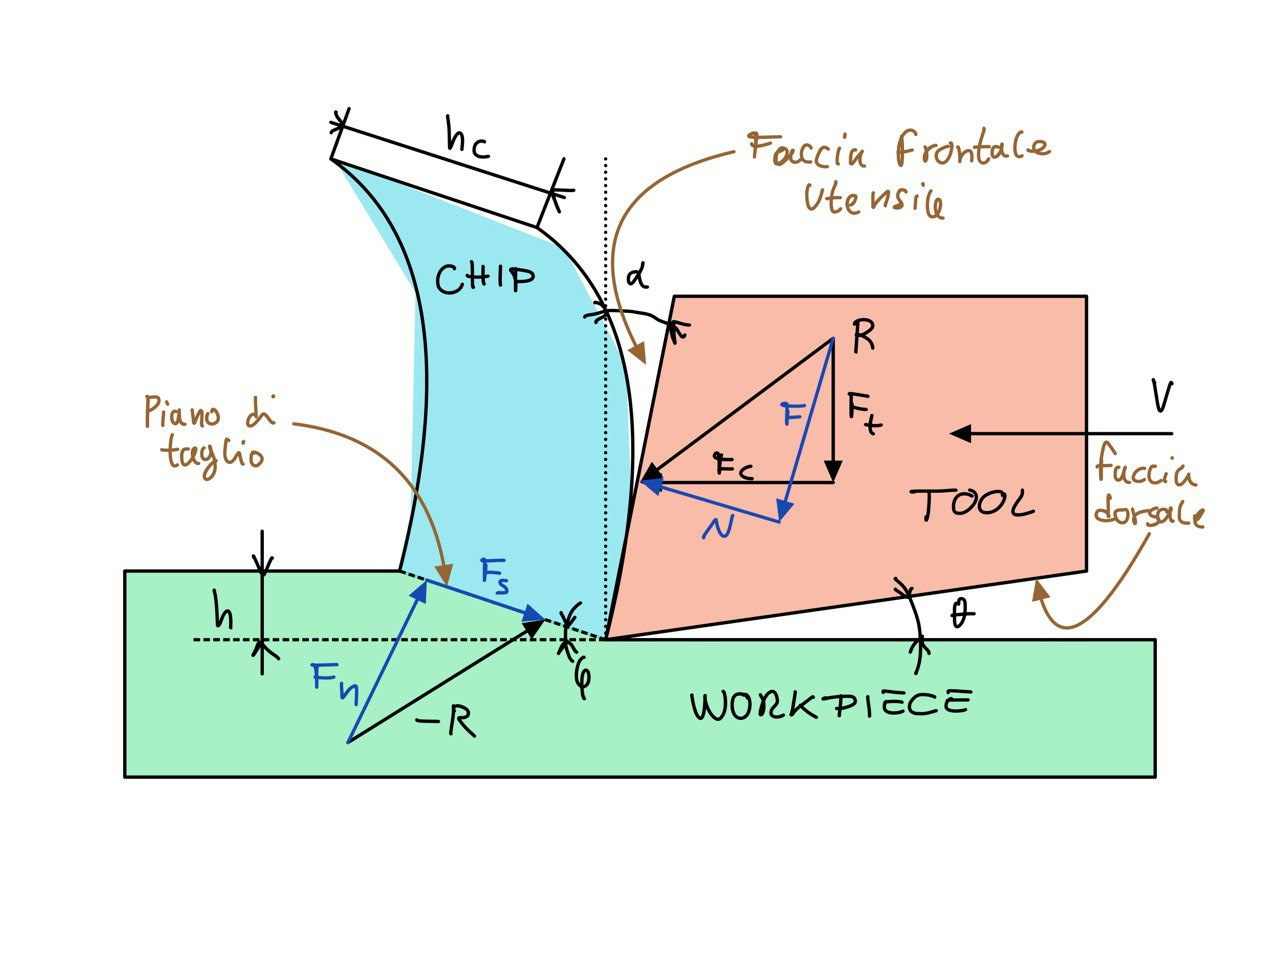
\includegraphics[width=0.7\textwidth]{TaglioOrtoScheme}}
\caption{Taglio Ortogonale}\label{fig:TaglioOrto}
\end{figure}
Si dice che il taglio è ortogonale quando la lama dell'utensile è ortogonale alla direzione della velocità di taglio.
Allora si possono definire diversi parametri come riportato nella definizione \ref{def:ParamTaglioOrto}.

\begin{definition}{Parametri del taglio ortogonale}{pramTaglioOrto}
\begin{description}
\item[$\alpha$] Angolo di spoglia superiore o frontale. Da cui
	\begin{description}
	\item[Se $\alpha > 0$] allora si dice che l'utensile ha angolo acuto,
	\item[Se $\alpha < 0$] allora si dice che l'utensile ha angolo ottuso.
	\end{description}
\item[$\theta$] Angolo di spoglia inferiore
\item[$\phi$] Angolo di taglio
\item[$h$] Spessore di taglio indeformato
\item[$h_c$] Spessore del truciolo
\end{description}
\label{def:ParamTaglioOrto}
\end{definition}

Come ipotesi ideale, si considererà che tutta la deformazione del materiale avverrà
solamente sul piano di taglio.
Allora, dai parametri del taglio ortogonale si possono ottenere:
\begin{equation}
r_c = \frac{h}{h_c} = \frac{l_c}{l} := \text{Rapporto di taglio}
\end{equation}
Dove:\\
\begin{tabular}{cl}
$l_c$ & è la lunghezza del truciolo\\
$l$ & è la lunghezza del taglio\\
\end{tabular}
\\
Mentre:
\begin{equation}
F = K \cdot A
\end{equation}
ovvero, la forza necessaria a tagliare il pezzo sarà proporzionale all'area $A$ del piano di taglio 
dovuta dalla lunghezza del piano stesso per la profondità del pezzo in senso ortogonale alla 
figura \ref{fig:TaglioOrtoParam}; in più sarà proporzionale alla pressione $K$ esercitata dall'utensile sul pezzo
Inoltre, si può intuire che: per abbassare l'intensità della forza complessiva per il taglio
sarebbe opportuno aumentare $\phi$, così da limitare l'estensione del piano di taglio e di 
conseguenza la sua area.
Si può ottenere una stima dell'angolo di taglio tramite
\begin{equation}
\tan\phi = \frac{r_c \cos\alpha}{1-r_c\sin\alpha}
\end{equation}
considerando che il rapporto di taglio lo si può misurare abbastanza facilmente dato che:
lo spessore di taglio lo si decide in base alla lavorazione da effettuare, mentre lo
spessore del truciolo lo si può misurare abbastanza facilmente.
Dunque è evidente che l'angolo $\alpha$ lo si vuole molto grande, in modo da generare piani
di taglio molto piccoli: garantendo la necessità di applicare una forza minore.

Risulta utile prestare attenzione alla successiva considerazione.
Il valore di deformazione che si raggiunge con le lavorazioni per asportazione di truciolo
è nettamente più alte che non le deformazioni per lavorazioni tramite deformazione.
Giusto per dare un'idea dell'ordine di grandezza:
\begin{equation}
\dot{\gamma} = \frac{v_s}{d} = \frac{\cos\alpha}{\cos\left(\phi - \alpha\right)} \frac{v}{d} \left[\unit{\s^{-1}}\right]
\end{equation}
nella tecnica, si osservano i seguenti valori:
\begin{description}
\item[Lavorazione per deformazione] $\approx 1 \div 10 \left[\unit{\s^{-1}}\right]$
\item[Lavorazione per asportazione] $\approx 1000 \left[\unit{\s^{-1}}\right]$
\end{description}

\subsection{Fattore di attrito}
Sappiamo che il fattore di attrito ricopre importante ruolo per quanto riguarda questo tipo
di lavorazioni. Ci si deve prestare attenzione.

\begin{equation}
\mu = \frac{\tau_i}{p}
\label{eqn:FattoreAttritoIndef}
\end{equation}
Di base, questa sarebbe la definizione principale di fattore di attrito.
Si nota che passata la tensione tangenziale di Von Misess, 
l'attrito tende a calare, nonostante nell'equazione non sia previsto tale 
comportamento.
Ciò è dovuto al fatto che per calcolare il fattore di attrito si considera un materiale
indeformabile, quando nella realtà del taglio ortogonale, non può essere.
Dunque il materiale sarà \textbf{indeformabile} fino alla tensione di Von Misess, 
passata quella bisogna considerarlo \textbf{deformabile}.
Perciò l'equazione \eqref{eqn:FattoreAttritoIndef} non descrive completamente il comportamento.
Si è sviluppato un \texttt{fattore di attrito} adatto a tale fenomeno:
\begin{equation}
m = \frac{\tau_i}{K}
\label{eqn:FattoreAttritoDef}
\end{equation}
Dove $K$ è la tensione tangenziale all'interfaccia truciolo-utensile.
Nella pratica viene preferito il fattore descritto dalla \eqref{eqn:FattoreAttritoDef} 
perché più facile da calcolare. Oltre al fatto che permette di descrivere correttamente
il fenomeno dello \eng{sticking}.

\begin{definition}{Sticking}{*}
Fenomeno di aderenza tra il truciolo e l'utensile. 
\end{definition}

\subsection{Valutazione delle forze}
Per la valutazione delle forze messe in gioco per tale lavorazione si considereranno
i tre attori separatamente e man mano sovrapponendone gli effetti.

\begin{figure}
\centering
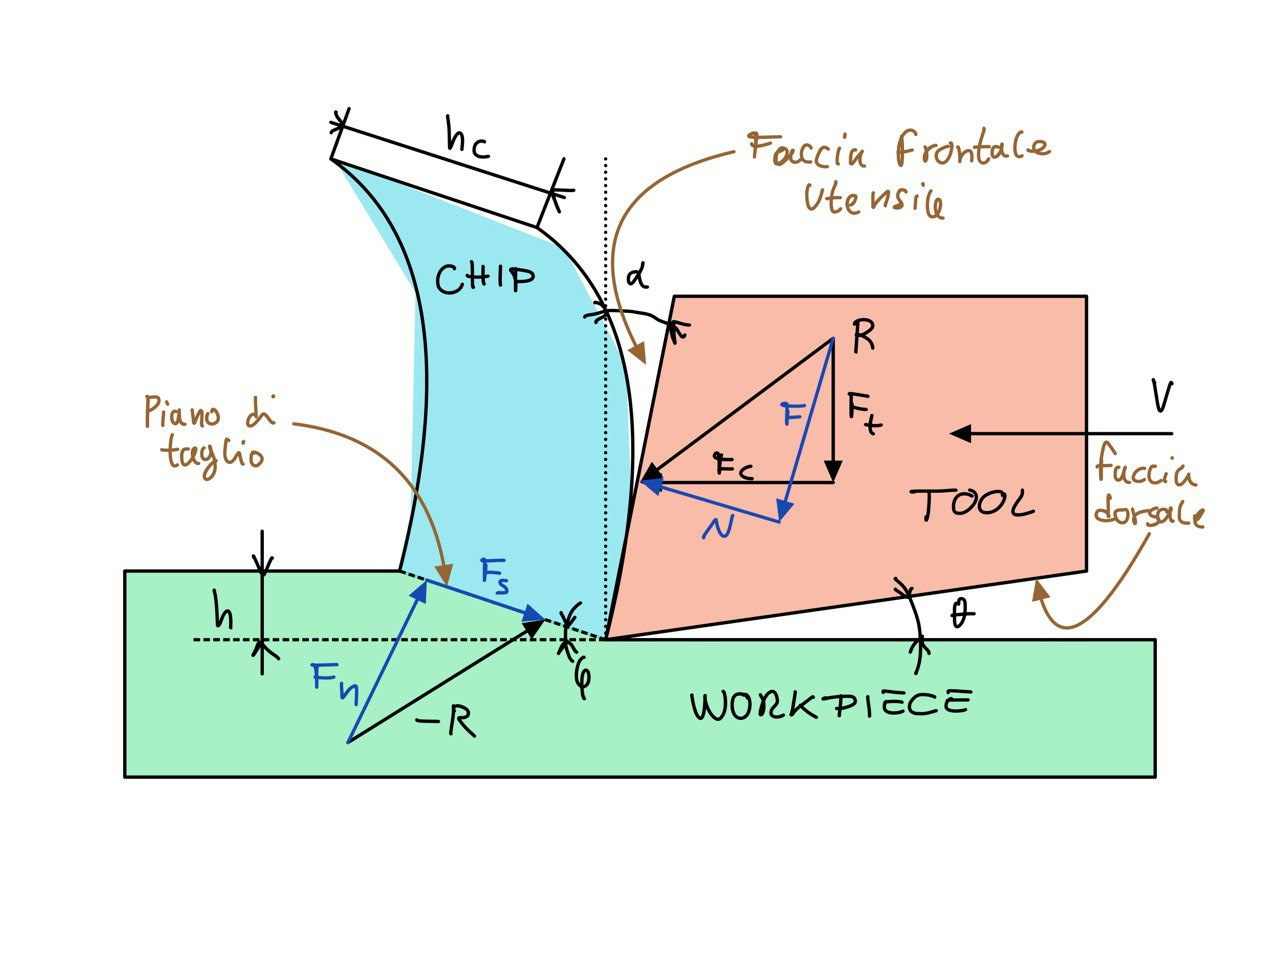
\includegraphics[width = \textwidth]{TaglioOrtoScheme}
\caption{Scomposizione delle forze per il taglio ortogonale}
\label{fig:TaglioOrtoForces}
\end{figure}

\subsubsection*{Porta utensile}
Considerando la scomposizione delle forze della figura \ref{fig:TaglioOrtoForces}.
Al porta utensile si può, operativamente, applicare una cella di carico per 
valutare la risultate applicata. Celle di carico più moderne possono eventualmente
valutare già le componenti di tale risultante.
allora possiamo ottenere i moduli delle forze:
\begin{equation}
\begin{cases}
F_c = R \cos(\alpha + \psi) &\text{Forza di taglio}\\
F_t = R \sin(\alpha + \psi) &\text{Forza di spinta dell'utensile}
\end{cases}
\end{equation}
Si possono definire ulteriori scomposizioni di forze: se prima la scomposizione
avveniva su proiezioni degli assi di riferimento rispetto al pezzo lavorato; ora si 
possono definire delle scomposizioni rispetto all'utensile.

\subsubsection*{Utensile}
Sempre in riferimento alla figura \ref{fig:TaglioOrtoForces}.
\begin{equation}
\begin{cases}
N = F_c \cos\alpha - F_t\sin\alpha\\
F = F_c \sin\alpha - F_t\cos\alpha
\end{cases}
\end{equation}
L'angolo relativo tra $R$ e $N$ viene indicato con $\beta$ e viene definito come 
\textbf{angolo d'attrito sulla faccia dell'utensile}. Vale:
\begin{equation}
\beta = \frac{F}{N} \approx \mu
\label{eqn:AngAttrito}
\end{equation}
Notare che $\beta$ è una sottospecie di coefficiente di attrito, infatti dipende
proprio da quest'ultimo.

\subsubsection*{Pezzo lavorato}
Lato pezzo lavorato si può vedere la totalità delle forze in gioco.
in particolare si devono evidenziare le forze:
\begin{description}
\item[$F_n$] risulta essere un contributo idrostatico per il materiale, dunque ne aumenta la 
duttilità. Aspetto che rende il taglio più difficoltoso. 
Ciò si risolve aumentando l'angolo del piano di taglio $\phi$ che si vedrà successivamente.
\item[$F_s$] è la vera e propria forza resistente al taglio. Si sviluppa come relazione della 
pressione di taglio resistente del materiale e l'area del piano di taglio.
\begin{equation}
F_s = k \cdot A
\end{equation}
Per rendere il taglio più agevole, si può ridurre l'area del piano di taglio nei modi che vedremo in seguito.
\end{description}

Riprendendo l'angolo del piano di taglio $\phi$, si hanno migliori condizioni lavorative
nel caso questo risulti essere molto grande.
Dalla letteratura si evidenziano le seguenti relazioni tra i vari angoli scomponenti le 
forze viste fino a prima:
\begin{subequations}
\label{eqn:Phi}
\begin{align}
\phi &= 45\unit{\degree} - \frac{1}{2}(\beta - \alpha) \label{eqn:Phi1}\\
\phi &= 45\unit{\degree} - (\beta - \alpha)\label{eqn:Phi2}
\end{align}
\end{subequations}
Sebbene indichino la relazione degli stessi parametri con due relazioni differenti \eqref{eqn:Phi}, entrambe hanno uno scopo preciso e nascono da considerazioni differenti.

\begin{description}
\item[\eqref{eqn:Phi1}] Si sviluppa partendo dalla considerazione che il sistema tenda
a consumare la minima energia.
\item[\eqref{eqn:Phi2}] Viene detta di \eng{Upper Bond}: ovvero ha l'obbiettivo di valutare
la massima forza necessaria per eseguire il taglio.
\end{description}

Per entrambi i casi risulta evidente che per aumentare $\phi$ si possono percorrere due strade:
\begin{description}
\item[$\searrow \beta$] siccome $\beta$ dipende dall'attrito tra truciolo e utensile, 
indipendentemente dallo \eng{sticking}, si può abbassare come angolo lubrificando 
l'interfaccia tra i  due.
\item[$\nearrow \alpha$] Aumentare l'angolo della faccia dell'utensile non è sempre una strada
percorribile, infatti si avrebbero utensili molto fini e fragili che tenderebbero a consumarsi
molto facilmente.
\end{description}

\begin{figure}
\centering
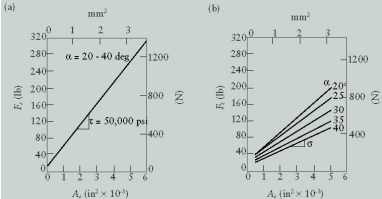
\includegraphics[width=\textwidth]{GraficiTaglioOrto}
\caption{Andamenti delle forze per il taglio ortogonale}
\label{fig:GarficiTaglioOrto}
\end{figure}

Nel grafico \ref{fig:GarficiTaglioOrto}.(a) è rappresentato l'andamento della forza di taglio 
$F_s$ giacente sul piano di taglio. Si osserva che tale forza aumenta all'aumentare dell'area 
del piano di taglio. 
Dunque è importante diminuire proprio quest'ultima: attraverso le strategie per 
aumentare $\phi$ viste in precedenza. Oltretutto tale andamento non è influenzato 
dall'angolo di spoglia superiore.
L'ipotesi che porta a tale costruzione sta nel fatto che il materiale è supposto non
incrudente. Infatti: raggiunto tale valore di sforzo tangenziale $\tau$ il materiale si 
rompe. Nel caso di materiale incrudente: si avrà una curva più che lineare, in quanto la 
deformazione porterà all'irrigidimento nella zona di taglio che necessiterà di maggiore
forza per avere la separazione del materiale.

Nel grafico \ref{fig:GarficiTaglioOrto}.(b) viene rappresentata la forza normale al piano di 
taglio $F_n$.
Questa dipende dall'angolo di spoglia superiore.
L'effetto di tale forza è stato già evidenziato: questa fornisce una specie di compressione 
idrostatica sul piano di taglio portando il materiale ad essere più duttile.
Ciò spesso si traduce in un truciolo continuo che però da una finitura superficiale peggiore.
\todo{\\Rivedere dopo aggiornamento sul truciolo}

\begin{figure}
\centering
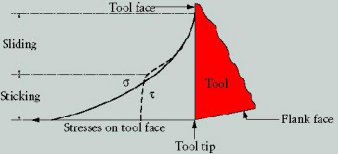
\includegraphics[width=\textwidth]{Sticking}
\caption{Tipologia di forze prementi sulla faccia dell'utensile}
\label{fig:sticking}
\end{figure}

Nel grafico \ref{fig:sticking} viene riportato il dettaglio sulla faccia superiore 
dell'utensile.
Si possono vedere due sezioni distinte:
\begin{description}
\item[\eng{Sliding}] in questa sezione si presenta lo scivolamento del truciolo sulla faccia
dell'utensile. Questo porta una cera forza resistente contro l'utensile di tipo $\tau$: ovvero 
di sforzo tangenziale. Si ha uno strisciamento completamente regolato dal coefficiente di 
attrito. Tale resistenza si annullerà nel momento in cui c'è distaccamento tra truciolo e 
faccia.
\item[\eng{Sticking}] nella zona di adesione si manifesta un particolare fenomeno per cui
il materiale del lavorato si accumula sulla punta dell'utensile. Ciò permette di generare una 
zona di ristagno che favorisce la separazione del materiale tra quello tagliato e il
truciolo. Di fatto in alcune occasioni può essere benefico per il tagliente in quanto
diventa uno strato protettivo. La resistenza portata da tale fenomeno diventa di pura 
deformazione $\sigma$. 
\end{description}

Al momento non si è ancora approfondita la finalità dell'angolo di spoglia inferiore $\theta$.
Idealmente servirebbe ad evitare lo strisciamento tra utensile e lavorato.
Siccome nella realtà bisogna considerare anche il ritorno elastico, non è possibile ottenere
un perfetto distaccamento tra utensile e lavorando. Dunque un po' di strisciamento si 
verifica in qualsiasi occasione. Ciò provoca usura dell'utensile.
Tra l'altro questo tipo di usura è la più severa per l'utensile.


\section{Taglio ortogonale realistico}